\documentclass{article}
\usepackage[spanish]{babel}
\usepackage {graphicx}
\graphicspath{ {images/} }
\usepackage{csquotes}
\usepackage{hyperref}
\usepackage[backend=biber, style=numeric]{biblatex}
\addbibresource{referencias.bib}
\title{Modelado y Programación, Proyecto 2: Base de Datos Musical}
\author{Mayté García Franco}
\date{Noviembre 2026}
\begin{document}

\maketitle

\section{Resumen}

En este segundo proyecto de Modelado y Programación se pidió crear una base de datos músical con interfaz. Aquí los usuarios podrán minar un directorio y se mostrará en la interfaz una lista de las canciones guardadas en la base de datos. Podrán editar la información de las cancione, artistas y albums, así como crear artistas, ya sean solistas o grupos. De igual forma, se podrán realizar consultas en esta interfaz, preferiblemente con un compilador básico. 

\section{Introducción}

Para este proyecto, el principal nuevo conocimiento adquirido fue la creación de una interfaz. Fue todo un proceso con altibajos ya que hubo momentos donde se volvía sencillos y otros donde volvía a complicarse, pero puedo decir que estoy satisfecha con esta primera interfaz que creé.

Así como en el primer proyecto, se aprendió un nuevo lenguaje de programación, que en este caso fue C++. Además de su uso tan sencillo debido a su parecido con Java, me pareció un lenguaje interesante debido a las estructuras y, específicamente para este proyecto, por el uso de Qt para la interfaz. Este lenguaje de programación también me empujó a usar un sistema de construcción que no había usado con anterioridad.

\section{Análisis y Diseño}

\subsection{División del problema}

Ya con la experiencia previa del proyecto del Chat, lo primero a hacer fue dividir lo más posible el problema, intentando tomar en cuenta tantos aspectos como sea posible. Este análisis resulto de la siguiente forma: 

\begin{itemize}
  \item Minero: recorre un directorio (recursivo) y lo guarda en la BD. Usa algún framework para recorrer directorios y para SQL. Necesita:
  \begin{itemize}
    \item Directorio
    \item BD: necesita: encuentraBD (acción: existe o no existe la bd), existeCancion (acción: la canción está en la bd. Necesita: dirección a revisar), directorio donde buscar, nombre BD / archivo con BD
    \item Acción - obtenerInfoCancion: necesita: dirección del archivo, título, artista, album, núm. de canción en el álbum, año, género
    \item Acción - agregarCancion: Necesita: BD
    \item Acción - agregarArtista: Necesita: artista, BD
    \item Acción - agregarAlbum: Necesita: BD
  \end{itemize}

  \item Compilador:
  \begin{itemize}
    \item Lee instrucción: Necesita: instrucción, analizar que la gramática es correcta (necesita la gramática y la instrucción), analizar que no modifique la base de datos.
    \item Traducir instrucción a SQL: Necesita: intrucción, gramática
  \end{itemize}

  \item BD:
  \begin{itemize}
    \item Acción - consulta
    \item Acción - modificarNombreTabla
    \item Acción - agregarNombreTabla
  \end{itemize}

  \item Vista:
  \begin{itemize}
    \item Accion - crearVista: necesita: todos los elementos de la interfaz. 
  \end{itemize}

  \item Controlador:
  \begin{itemize}
    \item Acción - detecta acciones en la vista: consulta, modificar album, modificar intérprete, modificar canción, agregar solista a banda, crear intérprete. 
  \end{itemize}
\end{itemize}

\subsection{Diseño de clases}

Ya con esta división, se pasó a hacer el diagrama de clases. El diagrama de clases que se muestra a continuación coincide con el programa final, por lo que es distinto al primer diagrama creado. De igual forma, hay clases que no muestran todos sus métodos por cuestiones de espacio, pero se muestran los que se consideran más importantes. (Figura 1)

\begin{figure}
  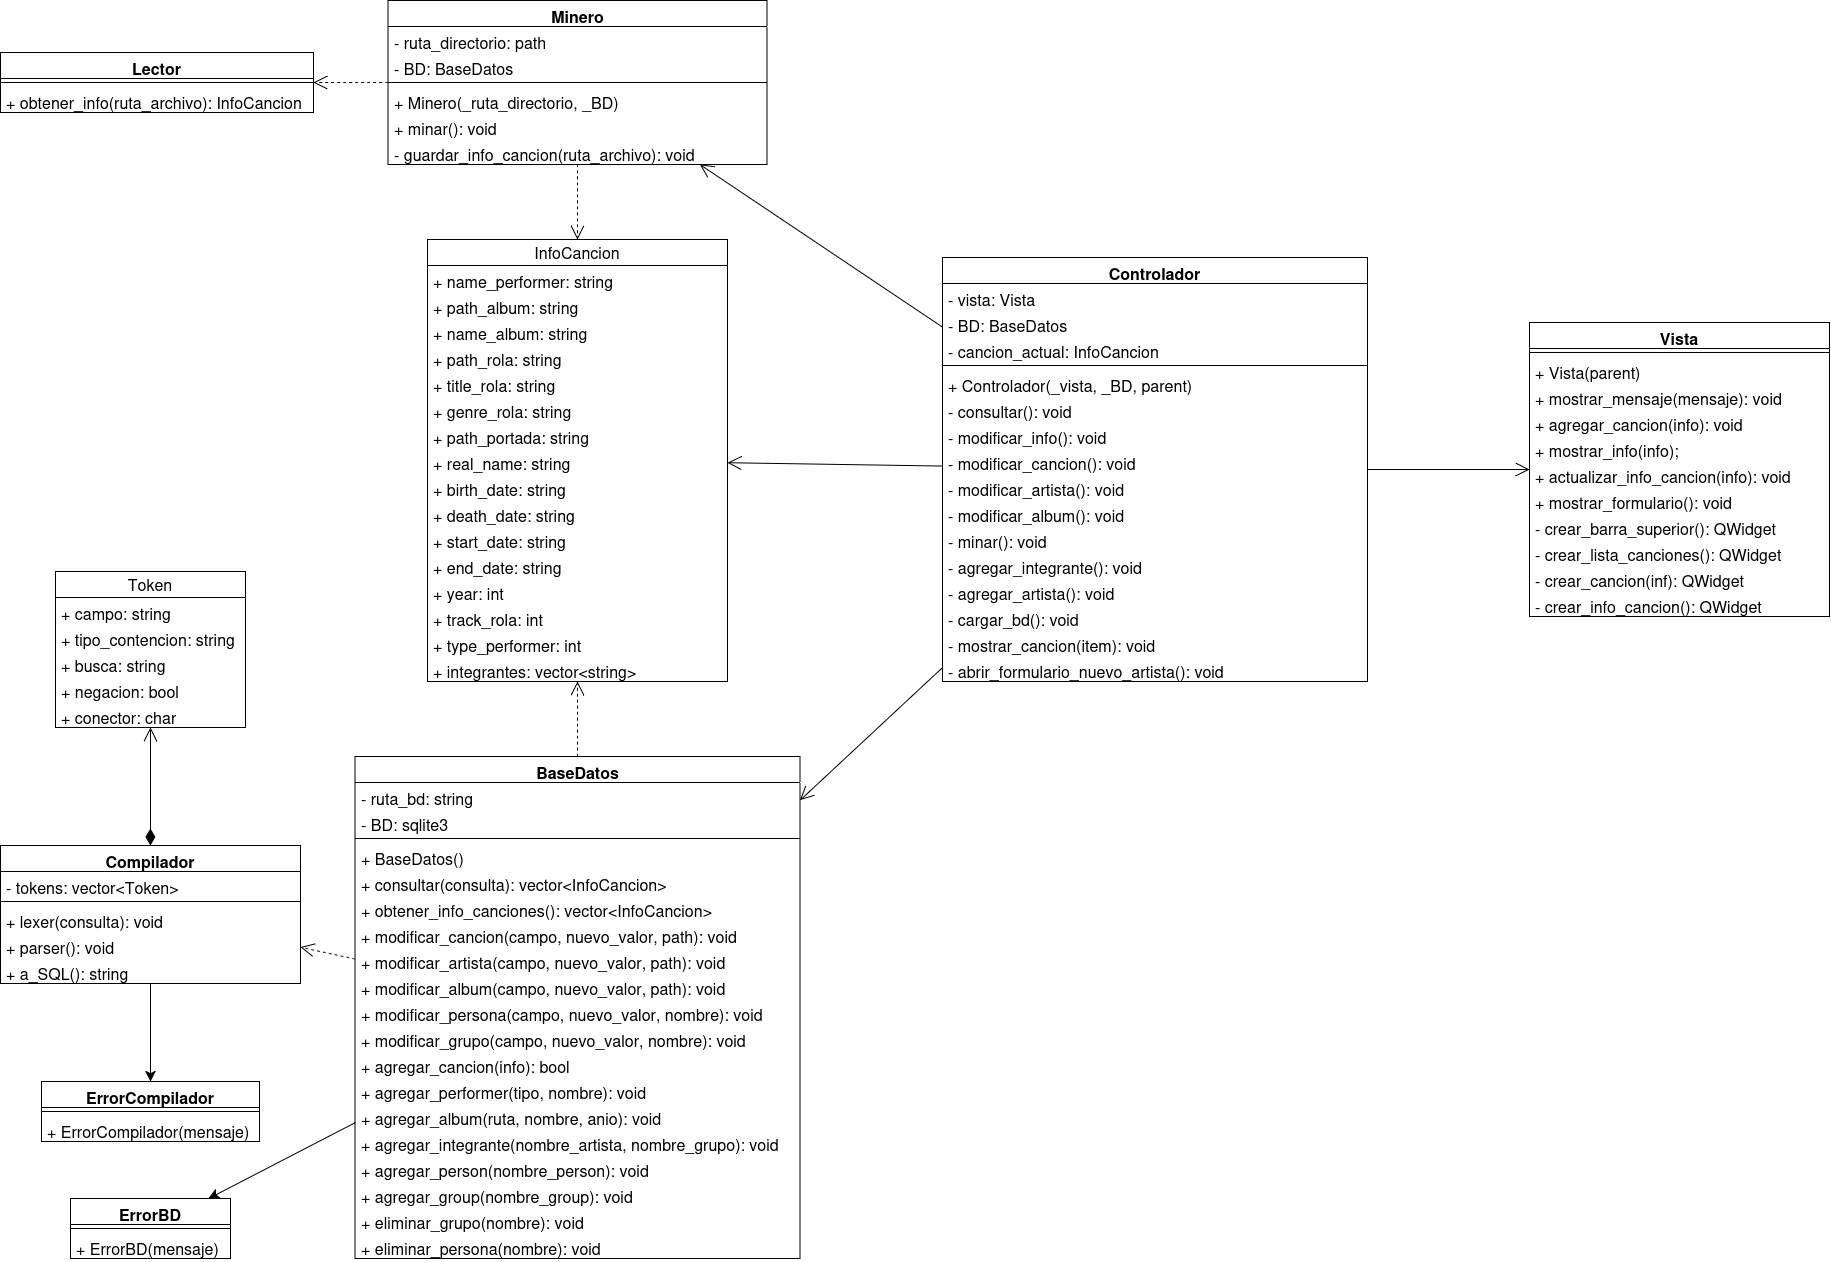
\includegraphics[scale=0.25]{Diagrama_De_Clases.png}
  \caption{Diagrama de clases.}
  \label{fig:diagrama_de_clases}
\end{figure}

\subsection{Diseño de la interfaz}

A continuación, se mostrará el diseño de la interfaz. Se basó levemente en la plataforma Soundcloud, buscando que sea algo sencillo de programar y de entender para el usuario. (FIgura 2)

\begin{figure}
  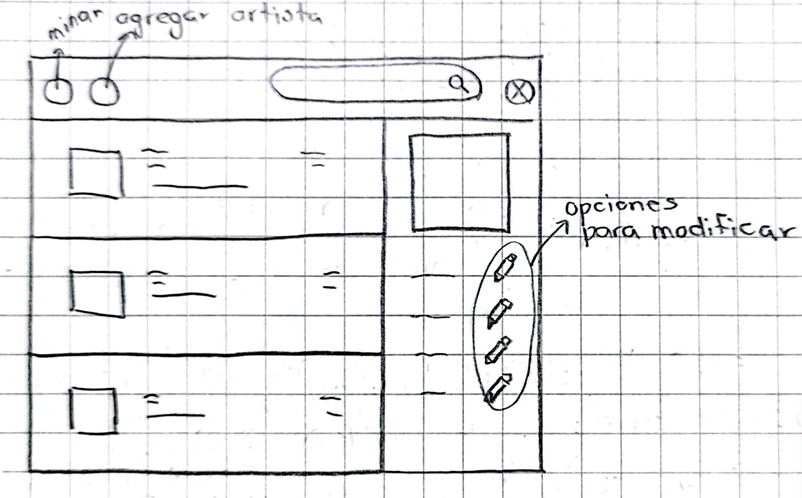
\includegraphics[scale=0.5]{Interfaz.png}
  \caption{Diseño de la interfaz.}
  \label{fig:diseño_interfaz}
\end{figure}

\section{Implementación}

Para este proyecto se decidió usar el lenguaje \textbf{C++}, esto debido a que en primer lugar se decidió usar Qt para crear la interfaz y este framework se basa principalmente en C++, por lo que usar este lenguaje para todo el programa facilitaría el desarrollo. A pesar de que esta fue la razón principal por la cual se tomó esta decisión, otro punto importante fue su parecido a Java, facilitando un poco más su rápido entendimiento.

En cuanto al sistema de construcción, se decidió usar \textbf{Meson} más que nada por curiosidad por probarlo. El proyecto pasado vi que varios lo usaron así que me dió curiosidad probarlo también.

Hablando un poco más sobre el framework para crear la interfaz, \textbf{Qt} se puede usar principalmente de dos formas: que uno haga directamente el programa de la interfaz en su editor de texto o usar Qt Creator. Intenté la segunda opción, pensando que sería más sencillo y rápido debido a la sección donde permite únicamente arrastrar elementos y así crear la interfaz. Lo estuve intentando durante un tiempo, pero sentí que no tenía mucho control en lo que hacía, sentía que sería más trabajo crear la interfaz ahí y después buscar como agregarla al proyecto, además de que darle propiedades a los objetos de la interfaz, tales como color, tamaño de letra, redondeado de orillas, etc., se volvía un reto debido a la confusión en como implementarlo en Qt Creator. Estos elementos me hicieron decidirme por la primera opción. A pesar de que se volvió complicado buscar información de como hacerlo debido a que la gran mayoría de la información que encontraba era específicamente para Qt Creator, después de lograr crear los primeros elementos se hizo mucho más sencillo el desarrollo y pude tener un control completo de lo que creaba. 

\section{Conclusiones}

Fue un proyecto bastante divertido, más que nada en la creación de la interaz y en su enlace con el Controlador. Fue muy emocionante ver como poco a poco la interfaz fue tomando forma y empezó a a funcionar conforme lo iba enlazando al controlador. Como mencioné en la sección anterior, fue difícil encontrar información de cómo usar el framework directamente y no por medio de Qt, pero una vez que encontré una fuente y empecé a crear la interfaz, fue sencillo seguir desarrollando por mi cuenta. También fue complicado encontrar como enlazar el controlador con la vista ya que encontraba que normalmente el controlador y la vista la hacían en un mismo archivo, pero una vez encontré como realizarlo fue muchísimo más sencillo.

El minado fue bastante sencillo con ayuda de la librería taglib. A pesar de mi análisis inicial donde dividí el minero en agregar canción, artista y álbum, después de un tiempo me di cuenta que crear la estructura InfoCancion no solo resultó mejor para guardar la información de las canciones y esto guardarlo en la base de datos, sino que facilitó el manejo de datos en todo el programa. Facilitó esta parte del minero, para modificar información en la base de datos o hacerle consultar y para que en la lista de la interfaz también se guardaran los datos y acceder a ellos facilmente.

En cuanto a la base de datos, en el análisis pensé que ya había abarcado todo lo necesario pero al agregarle funcionalidad a la interfaz me di cuenta de que me faltaron varios elementos, tales como obtener todas las canciones o eliminar algunos registros. El uso de prepare y bind siento que ayudó no solo a asegurar que se ejecute una instrucción de forma correcta, sino para hacerme entender con mucha mayor facilidad el código.

Finalmente, el compilador. No fue tan complicado de hacer, más que nada lo vi como leer poco a poco una cadena, identificar las partes importantes y acomodarlas de manera distinta para que se cree una consulta.

De forma general, siento que pude realizar mejor el análisis y diseño. Siento que mi planeación se cumplió esencialmente. El minero necesitó menos cosas de las que pensé, la base de datos solo necesitaba algunos métodos más, del compilador era más que nada el lexer, el parser y la traducción final. La vista no fue tanto como esperaba, no fue únicamente un método de crear vista, fueron más. Lo que sí pude seguir más fielmente fue mi idea inicial de cómo se vería la interfaz, por lo que me siento satisfecha.

Al inicio del proyecto sí me tardé en iniciarlo, pero siento que pude avanzarlo de forma constante. El primer proyecto lo terminé muy a las prisas, pero este lo terminé de forma mucho más tranquila, marcando una diferencia notable en qué tanto tiempo dediqué al proyecto.

\section{Bibliografía}

\nocite{*}
\printbibliography

\end{document}
